\chapter{System design}
\section{Overview}

In this chapter we will describe the design of the system from components and architectural point of view. The system design and architecture will rely on the requirements, actors and the enviroment described in precious chapters overall.The system is divided in components based on the development packages needed. This description will give enough information about the system and it's components and an overview on how the real world implementation will look like.

\section{Desgin goal}

\subsection{Robustness}
The system is decomposed in a way that each component can be contained in their separate processes where they can fail for their own with out causing the whole system to stop. All the components do their own validation to minimize system failure caused by bad input and data.

\subsection{Correctness}
The components will be able to tested individually for satisfying the business and development requirements. Then so we can refactor their internals easily and intuitively. The components will be verified for correctness with automated tests, run tests and code inspection by team and automated tools for standards.

\subsection{Flexibility}
When needs of the users and development team evolve the system will be easy to adapt to the new needs. Each and individual component contain their own separate logic and purpose, this makes each componenet easily extenible.

\subsection{Reusability}
The system is decomposed to be a set of components that can be used with different contexts and applications. We divided the main services as a component that can behave differently based on the configurations with out much alteration.

\subsection{Efficient}
Each component is designed in a way that can harness the power of modern machines with concurrency with much efficient parts of the system and cheaper execution based on the enviroment to be used. That includes good libraries and softwares that can run in embedded devices.

\subsection{Usability}
The components are designed to be responsive and usable for their respective stackeholders.

\section{System design}
	\subsection{System decomposition}

Kitab is composed of 4 components as shown in the graphic below. We decomposed the system to be separately maintained and developed, based on our skillset. Each component designed will have it's own service with it's responsibility to take care. In this way the system will be more realizable as different components. Figure~\ref{dia_sys_decomposition} shows how we decomposed kitab.

	\begin{figure}[H]
	\begin{center}

	\tcbox{\includegraphics[width=10cm]{"Diagram/System Decomposition".png}}
	\caption{System decomposition diagram for kitab}
	\label{dia_sys_decomposition}

	\end{center}
	\end{figure}

	\subsection{Module Description}

	\begin{description}
		\item[Content management] module handles the logic for managing contents and their data. 
		\item[User management] module handles the logic for managing user accounts and history, which helps in the recommentdation.
		\item[Kitab service] module handles the loadbalancing, routing and centeral database for the for different parts of the whole system.
		\item[Kitab app] module serves as an interface of the system to the different users. With this module the system is exposed to the external users.
	\end{description}

\section{Architecture}
	\subsection{Architectural Style and Pattern}

		\subsubsection{Architectural style}

		\begin{description}
			\item[Pipe-Filter architectural style] - is an architectural style in which different processing components form a chain so that the output of one component can be input to the following one.
			
			\item[Client-Server architectural style] - is an architectural style in which division of components where the client intiates a communication and requests different resources and the server responds to the request.
			
			\item[Publish-Subscribe architectural style] - is an architectural style in which senders of messages(publishers) publish messages with out knowing the recipient component.
		\end{description}

		\subsubsection{Architectural pattern}

		\begin{description}
			\item[Model-View-Controller architectural pattern] - This architectural pattern the main components in the system implementation are divided as :-
			\begin{description}
				\item[Model] - component that holds persistent data. \\
				In our case - database to store all the applications' data and it's abstraction as an ORM.
				\item[View] - component that works what the user will see and how the data could be presentable.\\
				In our case - interfaces for the web and mobile client application.
				\item[Controller] - component that controls the system state and interaction with the outside enviroment.\\
				In our case - the gin web server and buffalo router as a backend.
			\end{description}
			The figure~\ref{dia_mvc_arch_pattern} shows how "MVC" architectural pattern is used in the system.
		\end{description}

		\begin{figure}[H]
		\begin{center}

		\tcbox{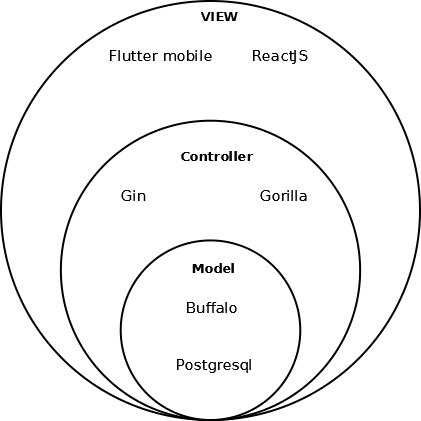
\includegraphics[width=7cm]{Diagram/MVC.png}}
		\caption{MVC architectural pattern for kitab}
		\label{dia_mvc_arch_pattern}

		\end{center}
		\end{figure}

      \pagebreak

      \subsection{Component Diagram}

      In the Unified Modeling Language(UML) a component diagram displays the high level structure of the whole system divided in to multiple components. It also describes the organization and connection of the physical components in the system. It helps model the implementation details and check that every aspect of the system's required functions is covered by planned development.

      \vspace{0.5in}

		\begin{figure}[H]
		\begin{center}

		\tcbox{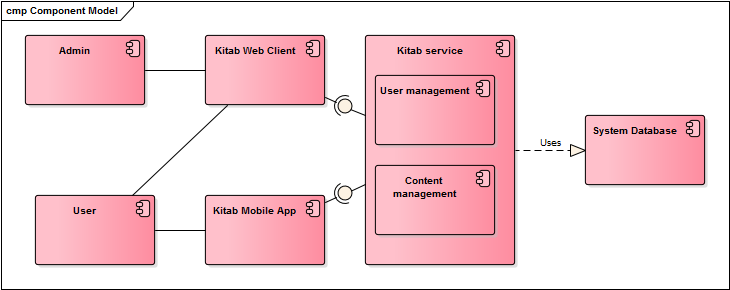
\includegraphics[width=\textwidth]{Diagram/Component.png}}
		\caption{Kitab Component diagram}
		\label{dia_mvc_cmpnt}

		\end{center}
		\end{figure}

      \pagebreak
      
      \subsection{Deployment Diagram}

      In the Unified Modeling Language(UML) a deployment diagram displays the physical arrangement of hardware and software execution components and the middleware between them while the system is deployed. Figure~\ref{dia_mvc_dplymnt} shows how the kitab system is arranged during deployment.

      \vspace{0.5in}

		\begin{figure}[H]
		\begin{center}

		\tcbox{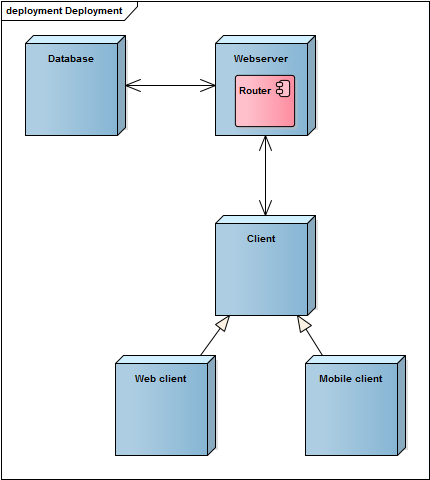
\includegraphics[width=\textwidth]{Diagram/Deployment.png}}
		\caption{Kitab Deployment diagram}
		\label{dia_mvc_dplymnt}

		\end{center}
		\end{figure}

\section{Database design}

	\begin{figure}[H]
	\begin{center}

	\tcbox{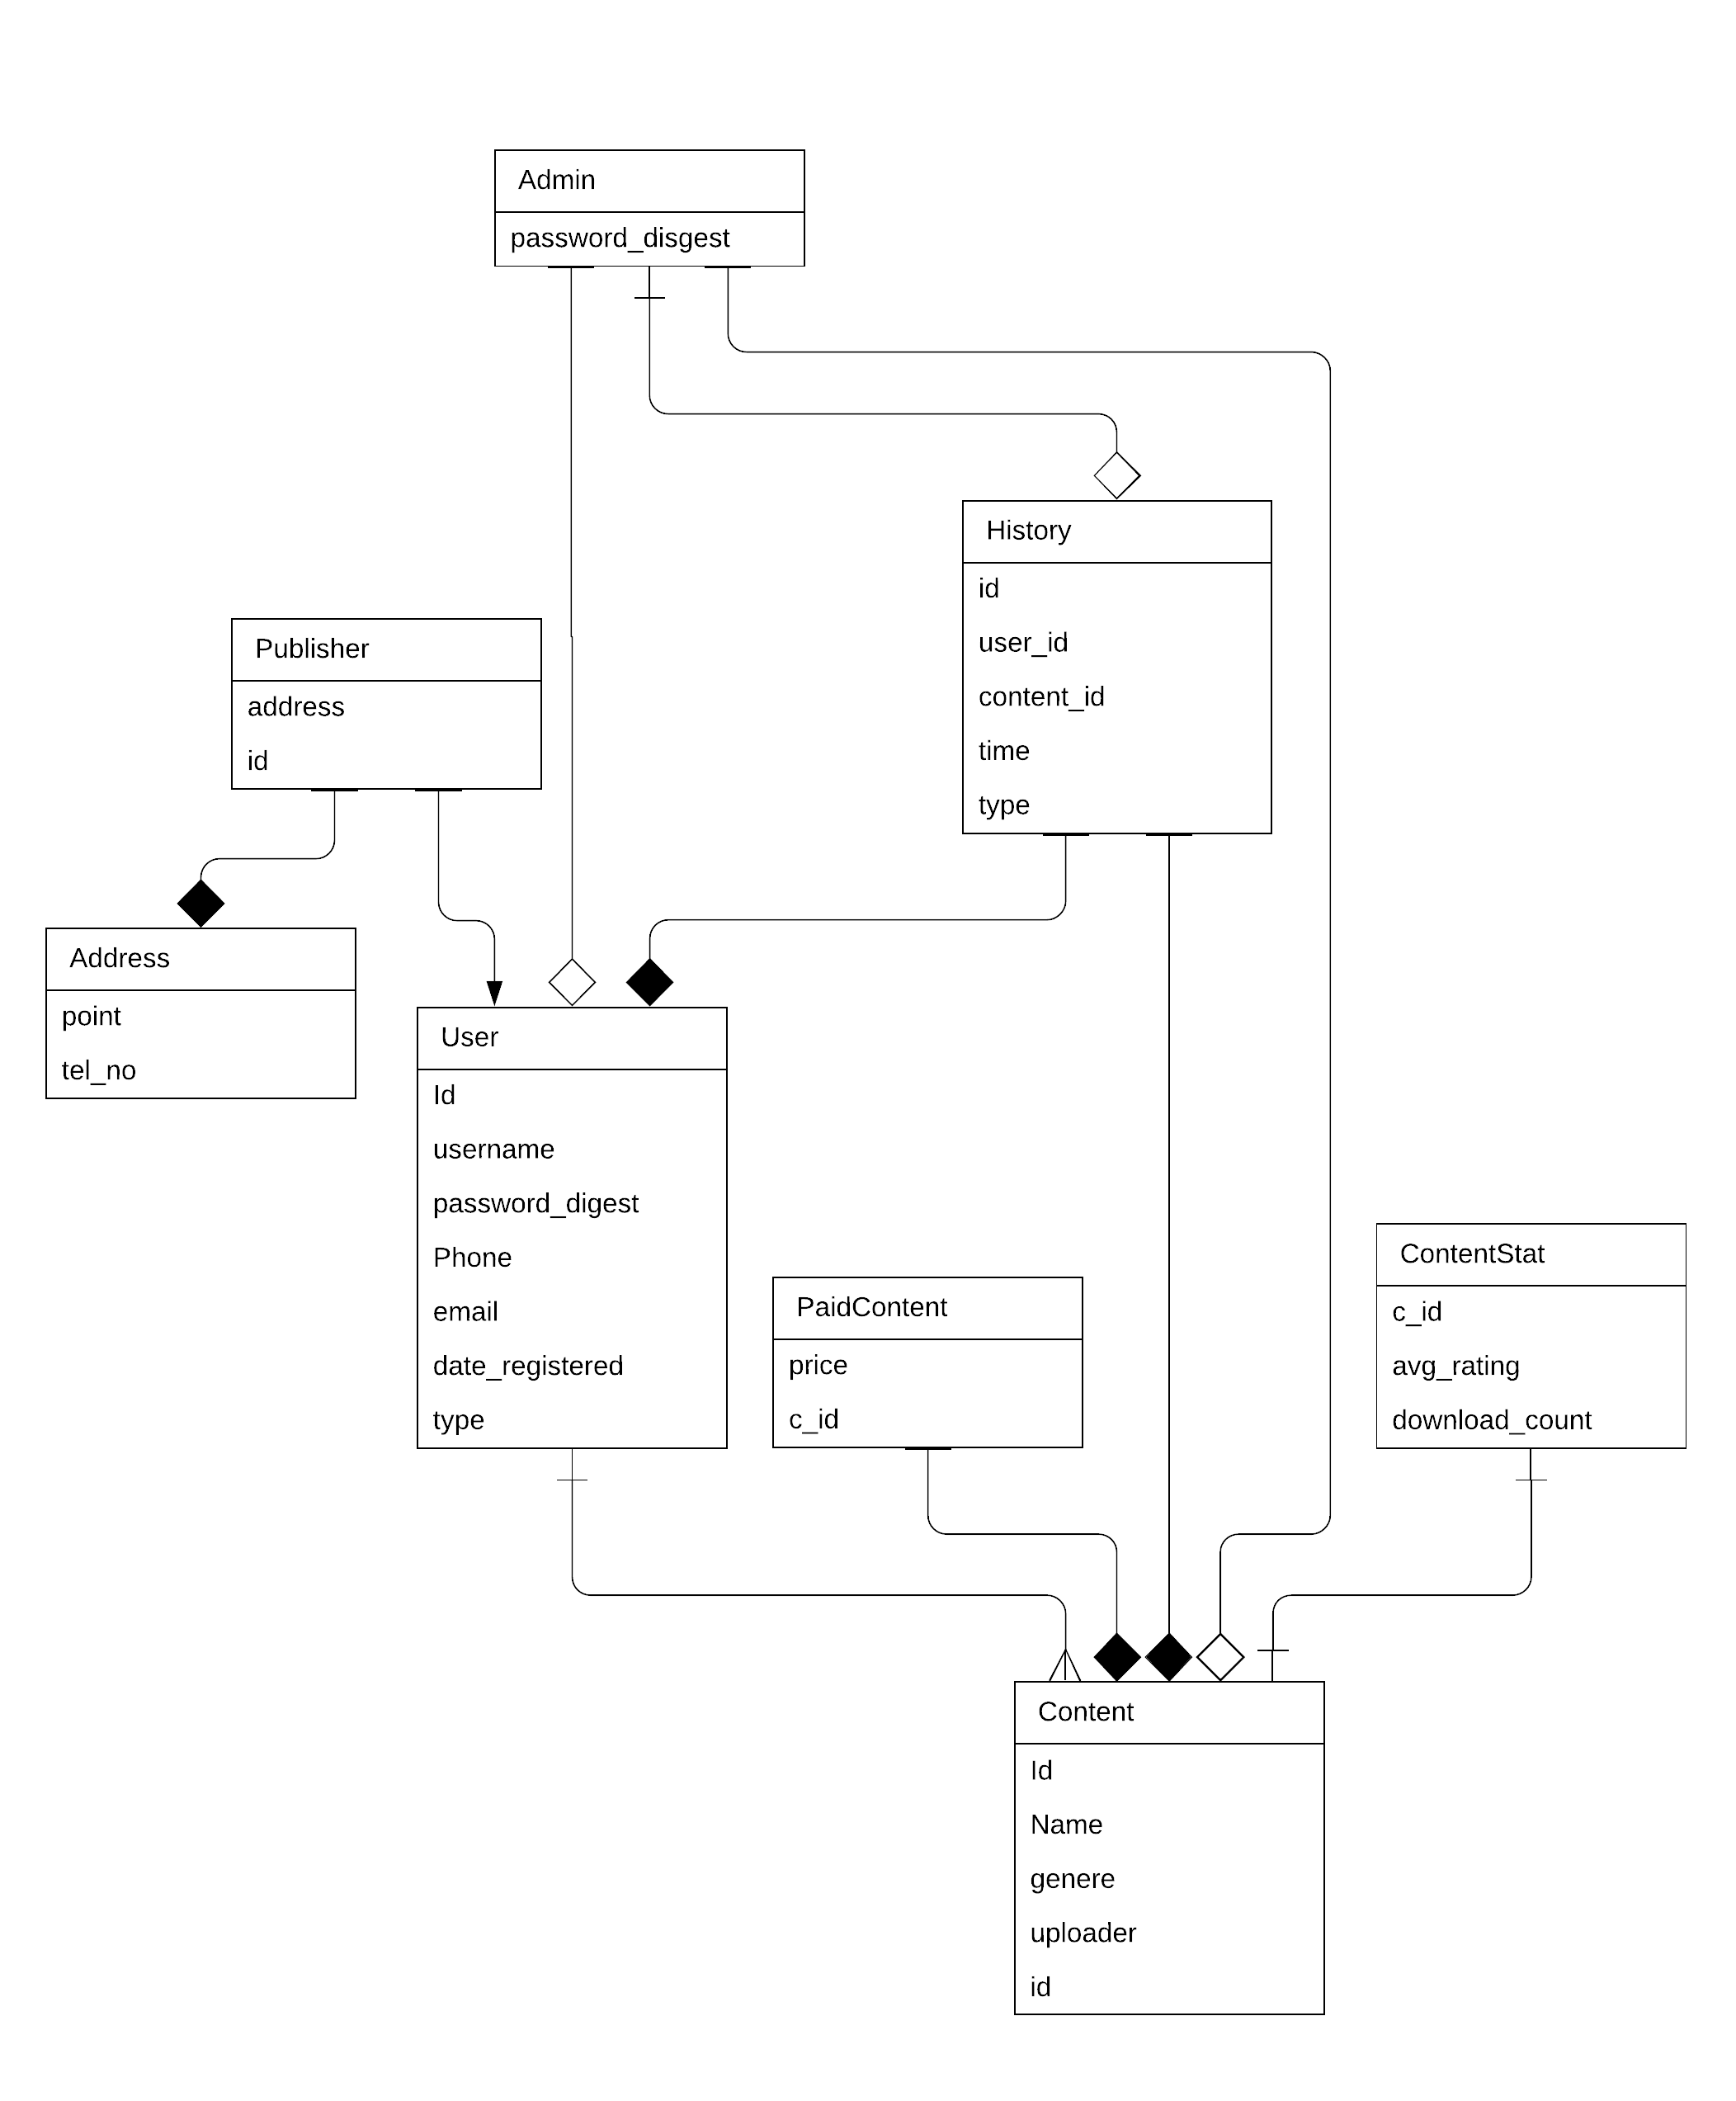
\includegraphics[width=0.9\textwidth]{Diagram/ER.png}}
	\caption{Kitab Entity Relationship diagram}
	\label{dia_er}

	\end{center}
	\end{figure}


% \section{User-interface design}